%--------------------------------------------------------------------------------


\documentclass[12pt]{article}
\usepackage[T1]{fontenc}
\usepackage[labelsep=period]{caption}

\usepackage[all]{hypcap}
\usepackage[utf8]{inputenc}
\usepackage{graphicx}

\usepackage[english]{babel}
\selectlanguage{english}

\usepackage{subfig}
\usepackage{color}
\usepackage{url}

\usepackage{hyperref}
\hypersetup{colorlinks=false, linkbordercolor=1 1 1, citebordercolor=1 1 1}

\usepackage[right]{lineno}
\usepackage{titling}
\renewcommand\linenumberfont{\normalfont\tiny\color{blue}}

\title{Computer Vision Course}
\author{Emanuele Corongiu <xcoron02@stud.fit.vutbr.cz>}
\date{\today}
\maketitle

%--------------------------------------------------------------------------------


\begin{document}
\selectlanguage{english}


\section{Abstract}
In this work, an attempt was made to train a YOLO (You Only Look Once) model for the purpose of recognizing and tracking car license plates. The model was trained under different conditions in order to appreciate some differences in its results.

%%%%%%%%%%%%%%%%%%%%%%%%%%%%%%%%%%%%%%%%%%%%%%%%%%%%%%%%%%%%%%%%%%%%%%%%%%%%%%%%%%%%%%%%

\section{Yolo V8}

\section{Dataset}
Presentazione dei dataset utilizzati e dei risultati ottenuti da loro, guardare su roboflow.



\begin{equation}
  \label{moje-rovnice}
  c = a + b
\end{equation}

sdfsdfsdfsdf \ref{fig:obrazek} sdfsdfsdfsdf

\begin{figure}[htb]
  \centering
  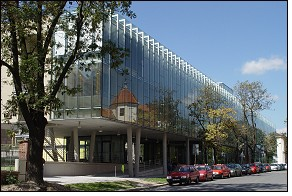
\includegraphics[width=5cm,keepaspectratio]{obrazek.jpg}
  \caption{try \cite{wikipedia}}
  \label{fig:try}
\end{figure}


%%%%%%%%%%%%%%%%%%%%%%%%%%%%%%%%%%%%%%%%%%%%%%%%%%%%%%%%%%%%%%%%%%%%%%%%%%%%%%%%%%%%%%%%



\bibliographystyle{alpha}
\begin{flushleft}
  \bibliography{project}
\end{flushleft}

%\appendix
%\newpage
%\section{}

\end{document}
